% =============================================================================
\subsection{Melhores Configurações por Base e Modelo Global}
\label{sec:melhores}

Um dos princípios fundamentais evidenciados pela transição da Fase~1 para a
Fase~2 é a manifestação do teorema \emph{No Free Lunch}~\cite{wolpert1997no}:
intervenções algorítmicas que resolvem patologias severas em determinadas
paisagens podem introduzir ruído estrutural em outras. Ao todo, a Fase~2 avaliou
14 configurações algorítmicas distintas (além da referência da Fase~1), totalizando
1.350 execuções independentes organizadas por ablações isoladas e escadas
cumulativas de empilhamento. A partir desse espaço amostral estruturado, a análise
desdobra-se em duas diretrizes complementares: a determinação da \textbf{melhor
configuração especializada por base} e a identificação de uma \textbf{configuração
global de melhor compromisso}, eleita entre todas as variantes avaliadas.

% -----------------------------------------------------------------------------
\subsubsection{Melhor Configuração por Base e Justificativa Teórico-Experimental}
\label{sec:melhor_por_base}

A \cref{tab:melhores_por_base} sintetiza a configuração vencedora para cada
conjunto de dados, acompanhada do ganho empírico sobre a Fase~1 e das
expressões matemáticas simbólicas recuperadas.

\begin{table}[htbp]
  \centering
  \caption{Melhor configuração encontrada para cada base de dados (30 repetições).}
  \label{tab:melhores_por_base}
  \small
  \resizebox{\linewidth}{!}{%
  \begin{tabular}{@{}llcccccr@{}}
    \toprule
    Base & Melhor Configuração & RMSE teste (médio) & Mediana (IQR) & Mínimo & Tam. & $R^2_{\text{teste}}$ & Ganho vs F1 \\
    \midrule
    \code{synth1}    & \cfg{Stack~A2} ($\eps$-Lex + Dedup + Parcim. + Ops) & $\mathbf{0.69 \pm 1.81}$ & $\mathbf{0.093\ (0.76)}$ & 0.0006 & 35.9 & 1.00 & $-87.5\%$ (média) \\
    \code{synth2}    & \cfg{Stack~B3} ($\eps$-Lex + AQ + Scaling + Dedup + Parcim. + Ops) & $\mathbf{1.52 \pm 0.26}$ & $\mathbf{1.43\ (0.20)}$ & 1.2842 & 61.6 & 0.86 & $-93.9\%$ (média) \\
    \code{concrete1} & \cfg{Stack~B4} ($\eps$-Lex + AQ + Scaling + Dedup + Parcim. + Ops + Não-Lin.) & $\mathbf{7.72 \pm 0.64}$ & $\mathbf{7.60\ (0.74)}$ & 6.7621 & 43.3 & 0.78 & $-35.5\%$ (média) \\
    \bottomrule
  \end{tabular}}
\end{table}

\paragraph{\code{synth1}: \cfg{Stack~A2} e a Dedução Analítica da Função Alvo.}
\label{sec:melhor_synth1}

\paragraph{Identificação Empírica e Prova da Função Geradora.}
Diferente de cenários com modelos fenomenológicos conhecidos, a formulação exata
da base \code{synth1} não foi assumida \emph{a priori}, mas deduzida a partir dos
próprios resultados da regressão simbólica e verificada numericamente contra os
dados brutos. Na semente~0 do \cfg{Stack~A2}, o algoritmo convergiu para uma
árvore sintática compacta de apenas 27 nós com RMSE de teste de $\mathbf{0.000576}$:
\begin{align}
  \hat{y} &= \big(((0.2501 x_1) x_1 + ((0.2501 x_1) x_1 - x_1)) + (x_0^2 \cdot x_0^2)\big) - (x_0 \cdot x_0^2) \nonumber \\
          &= (0.2501 x_1^2 + 0.2501 x_1^2 - x_1) + x_0^4 - x_0^3 \nonumber \\
          &= x_0^4 - x_0^3 + 0.5002 x_1^2 - x_1.
  \label{eq:synth1_expr}
\end{align}
Observando que o coeficiente $0.5002$ é a soma de duas constantes efêmeras
sorteadas como $0.2501$ ($2 \times 0.2501 = 0.5002 \approx 1/2$), formulou-se a
hipótese da lei matemática exata subjacente:
\begin{equation}
  f(x_0, x_1) = x_0^4 - x_0^3 + 0.5 x_1^2 - x_1.
  \label{eq:synth1_ground_truth}
\end{equation}
A validação dessa expressão diretamente contra os arquivos originais do repositório
(\code{synth1-}\allowbreak\code{train.csv} e \code{synth1-}\allowbreak\code{test.csv}) confirmou a hipótese com rigor
matemático absoluto:
\begin{itemize}
  \item \textbf{No conjunto de treino (60 amostras):} a discrepância máxima
        $|y_i - f(x_{0,i}, x_{1,i})|$ é \textbf{exatamente 0.0}.
  \item \textbf{No conjunto de teste (600 amostras):} o erro absoluto máximo é de
        $\mathbf{8.88 \times 10^{-16}}$, correspondente ao piso da precisão de
        ponto flutuante de 64 bits (IEEE~754).
\end{itemize}
Essa verificação comprova categoricamente duas propriedades da base:
(i)~trata-se de um \textbf{polinômio de quarto grau} em $x_0$ e segundo grau em $x_1$,
com invariância em relação a $x_2$; e
(ii)~os dados foram sintetizados \textbf{sem nenhum ruído estocástico} ($\sigma_{\text{ruído}} = 0$).

\paragraph{Por que o \cfg{Stack~A2} é a Melhor Configuração?}
A elucidação da função alvo justifica teoricamente os resultados empíricos:
\begin{enumerate}
  \item \textbf{Prejuízo de graus de liberdade espúrios:} Como a resposta não
        possui desvios de escala e a forma funcional é puramente polinomial, a
        introdução de \emph{Linear Scaling} analítico (H6a) ou de primitivas
        transcendetais ($\log, \sqrt{\cdot}, \exp$; H6b) insere flexibilidade
        desnecessária. Dispondo de apenas 60 amostras de treino, essa flexibilidade
        conduz ao sobreajuste: ao habilitar H6b, a mediana do RMSE de teste piora
        severamente de $0.093$ para $2.24$ ($p = 7.7 \times 10^{-5}$).
  \item \textbf{Sinergia estrutural do \cfg{Stack~A2}:} A paisagem polinomial do
        \code{synth1} demandava: (a)~$\eps$-lexicase para manter linhagens
        especializadas em regiões do suporte; (b)~rejeição de clones (H3) para
        sustentar a diversidade na recombinação; (c)~parcimônia lexicográfica (H5)
        para extirpar \emph{introns} algébricos, viabilizando árvores mínimas; e
        (d)~mutação mista (H2), em especial a perturbação gaussiana sobre ERCs,
        permitindo que constantes convergissem suavemente para o valor analítico
        $0.25$ sem desmontar blocos polinomiais já formados.
\end{enumerate}
Nas 30 repetições independentes com o \cfg{Stack~A2}, \textbf{7 sementes alcançaram $\text{RMSE} < 0.01$}
e \textbf{15 alcançaram $\text{RMSE} < 0.1$} (mediana de $0.0933$ e mínimo de
$0.000576$), enquanto na Fase~1 nenhuma semente havia superado a barreira de $0.1$.

\paragraph{\code{synth2}: \cfg{Stack~B3} e o Fim das Explosões Assintóticas.}
\label{sec:melhor_synth2}

\paragraph{Por que é a melhor?}
A base \code{synth2} representa uma superfície racional que se anula ou
diverge nas proximidades do domínio. Sob a divisão protegida de Koza (Fase~1),
árvores geravam denominadores próximos de zero, explodindo fora da amostra de
treino ($415.3$ de erro máximo).

A combinação de \textbf{Analytic Quotient} (H1) com \textbf{Linear Scaling}
(H6a) formou uma sinergia indispensável: o AQ eliminou as assíntotas
verticais tornando toda a paisagem contínua e infinitamente diferenciável,
enquanto o \emph{Linear Scaling} absorveu analiticamente a amplitude da
superfície. A mutação mista (\cfg{Stack~B3}) forneceu o refinamento numérico
final, reduzindo a variância entre repetições para meros $0.2558$ e o erro
máximo de teste para $2.35$. O modelo \cfg{Stack~B4} adicionou operadores
transcendentais desnecessários, piorando a mediana de $1.43$ para $1.87$
($p = 3.8\times10^{-6}$).

\paragraph{Evidência Simbólica:}
O melhor indivíduo encontrado (semente~20, justamente a que explodia com erro
de $415$ na Fase~1) obteve RMSE de teste de $\mathbf{1.2842}$ com a seguinte
expressão suavizada:
\begin{equation}
  \hat{y} = 9.176 - 2.957 \cdot \mathrm{aq}\Big(x_0 + x_1 - 0.310 x_0 x_1, \, \Psi(x_0, x_1)\Big),
\end{equation}
em que $\Psi(x_0,x_1)$ é uma subárvore que modula continuamente a curvatura
sem nunca produzir divisão por zero.

\paragraph{\code{concrete1}: \cfg{Stack~B4} e a Modelagem de Relações Não-Lineares em Dados Multivariados.}
\label{sec:melhor_concrete}

\paragraph{Por que é a melhor?}
A base \code{concrete1} caracteriza-se como um problema empírico multivariado com
oito atributos contínuos de entrada ($x_0,\dots,x_7$) e uma variável alvo contínua $y$.
A análise exploratória dos dados revela duas particularidades que
impunham barreiras severas ao GP canônico avaliado na Fase~1:
\begin{enumerate}
  \item \textbf{Barreira de Escala (Média de $\bar{y} \approx 35.8$):} A variável resposta
        possui média amostral de $35.76$ e desvio-padrão de $16.27$. Em contrapartida,
        as constantes efêmeras (ERC) são sorteadas uniformemente no intervalo restrito
        $[-1, 1]$. Na Fase~1 (sem reescalonamento), os indivíduos precisavam acumular mais
        de 70 nós apenas somando e dividindo constantes para sintetizar a magnitude
        adequada da saída, esgotando o limite de profundidade 7 em nós estruturalmente
        triviais antes de conseguir modelar o relacionamento entre as variáveis.
  \item \textbf{Curvaturas e Saturações Não-Lineares Multivariadas:} Em conjuntos de
        dados tabulares com oito variáveis de dispersões distintas, as interações entre os
        atributos frequentemente exibem dinâmicas sublineares e amortecidas. O conjunto
        puramente aritmético $\{+,-,\times,\div\}$ é subexpressivo para reproduzir tais
        efeitos de saturação sem gerar polinômios de grau excessivo que provocam oscilações
        e inchaço descontrolado.
\end{enumerate}

O modelo \cfg{Stack~B4} contornou ambos os entraves de forma sinérgica:
\begin{enumerate}[label=(\roman*)]
  \item O \textbf{\emph{Linear Scaling} analítico (H6a)} via OLS calcula
        diretamente os coeficientes ótimos de translação ($\alpha \approx 22.4$) e
        amplificação ($\beta \approx 4.3$), desacoplando o ajuste de escala da busca
        estrutural e liberando a totalidade da árvore para mapear as dependências
        entre atributos;
  \item As \textbf{primitivas não-lineares protegidas (H6b)} ($\log, \sqrt{\cdot}, \exp$)
        oferecem uma base funcional natural para modelar efeitos amortecidos e
        não-lineares entre variáveis sem exigir árvores profundas, revertendo o
        subajuste estrutural;
  \item A \textbf{parcimônia lexicográfica (H5)} e o \textbf{AQ (H1)} garantiram
        expressões compactas com média de apenas $43.3$ nós (uma expressiva
        redução de $41.6\%$ em relação aos $74.1$ nós observados na Fase~1).
\end{enumerate}
O impacto prático dessa combinação foi expressivo: o coeficiente de determinação
saltou de $R^2 = 0.44$ para $\mathbf{0.78}$, a mediana do RMSE de teste caiu de
$11.81$ para $\mathbf{7.60}$, e a configuração superou o baseline da Fase~1 em
\textbf{30 de 30 sementes independentes} ($p_W = 1.9 \times 10^{-9}$).

\paragraph{Evidência Simbólica:}
A melhor expressão recuperada (semente~25, RMSE de teste $= \mathbf{6.7621}$ e
apenas 45 nós) ilustra como o algoritmo explorou as primitivas unárias para
sintetizar relações não-lineares com concisão:
\begin{equation}
\begin{split}
  \hat{y} &= 22.42 + 4.323 \cdot \Big[ \sqrt{-0.742 - x_1 + \log(x_6)} \\
          &\quad + \exp\big(\sqrt{\mathrm{aq}(1.155, x_4)}\big) \\
          &\quad + \mathrm{aq}\big(\mathrm{e}^{0.467} + x_1 + x_0, \, \log(-0.742 - x_7)\big) + \dots \Big],
\end{split}
\end{equation}
estabelecendo acoplamentos não-lineares entre múltiplos atributos
($x_0$, $x_1$, $x_4$, $x_6$, $x_7$) por meio de transformações logarítmicas e radicais.

% -----------------------------------------------------------------------------
\subsubsection{O Modelo Melhor Global: \cfg{Stack~B3} como Solução de Compromisso}
\label{sec:melhor_global}

\paragraph{O Dilema de Generalidade e a Racionalidade da Busca por Ablação.}
Se a regressão simbólica deve ser aplicada sobre um problema desconhecido no qual
a forma analítica e as propriedades da função subjacente não são acessíveis
\emph{a priori}, qual configuração algorítmica deve ser adotada?

Para responder a essa pergunta com rigor científico, é essencial explicitar o
espaço metodológico percorrido. Diante das seis hipóteses de intervenção
algorítmica investigadas na Fase~2 ($H_1$ a $H_6$), uma busca combinatorial
irrestrita de todas as combinações binárias possíveis ($2^6 = 64$) exigiria
avaliar $64 \times 3 \times 30 = 5\,760$ execuções completas de GP com 100 gerações,
totalizando mais de 57 milhões de avaliações de aptidão sintática.

Além do custo computacional proibitivo, a busca exaustiva por força bruta é
metodologicamente inadequada: a grande maioria das 64 combinações arbitrárias é
conceitualmente desarmônica ou antagônica. Por exemplo:
\begin{itemize}
  \item Introduzir primitivas não-lineares transcendentais ($H_{6b}$: $\log, \sqrt{\cdot}, \exp$)
        sobre a divisão protegida de Koza sem escalonamento linear ($H_{6a}$) e sem
        parcimônia ($H_5$) apenas multiplicaria explosões numéricas e inchaço de forma
        artificial, produzindo ruído estocástico sem valor analítico;
  \item Combinar modelos de ilhas ($H_4$) com altas taxas de mutação e sem filtragem
        de redundância sintática ($H_3$) apenas diluiria o gradiente seletivo da $\eps$-lexicase.
\end{itemize}

Por essa razão, a investigação adotou o protocolo padrão de \textbf{ablação
orientada a hipóteses e empilhamento cumulativo em escadas}
(\cref{sec:f2_ablacao}):
\begin{enumerate}
  \item \textbf{Ablação Isolada ($1 \times 1$ contra \cfg{S0}):} Cada mecanismo foi
        analisado isoladamente sobre o Estado Atual \cfg{S0} para mensurar sua
        contribuição marginal pura e sua significância estatística pareada
        (testes de Wilcoxon e Mann-Whitney). Mecanismos que aumentaram o custo de
        comunicação sem ganho estatístico de convergência (como o Modelo de Ilhas
        $H_4$) foram precocemente descartados (\emph{pruned});
  \item \textbf{Empilhamento Cumulativo em Escadas Lógicas:} Apenas as hipóteses com
        ganho comprovado foram compostas de forma ordenada ao longo de duas
        linhagens conceituais: a \textbf{Escada~A} (\cfg{Stack~A1} $\to$ \cfg{Stack~A2}),
        voltada à busca parcimoniosa e preservação de diversidade em superfícies
        polinomiais; e a \textbf{Escada~B} (\cfg{Stack~B1} $\to$ \dots $\to$ \cfg{Stack~B4}),
        orientada à eliminação de singularidades assintóticas, desacoplamento de escala
        via OLS e expansão de operadores.
\end{enumerate}

\paragraph{Clarificação Fundamental: Universo da Eleição do Modelo Global.}
É imperativo esclarecer que a eleição do \textbf{\cfg{Stack~B3}} como a melhor
configuração de compromisso geral \textbf{não é uma escolha restrita a um
confronto tripartite entre os três campeões locais} (\cfg{Stack~A2}, \cfg{Stack~B3}
e \cfg{Stack~B4}). Pelo contrário: a totalidade das \textbf{14 configurações
algorítmicas avaliadas na Fase~2} (além da referência canônica da Fase~1),
somando 45 matrizes experimentais e 1.350 execuções independentes, foi submetida
a um processo de ordenação e ranqueamento multiobjetivo simultâneo nas três bases
de dados.

A \cref{tab:ranking_global} reporta a síntese comparativa das configurações mais
relevantes ao longo de todas as bases, mensurando:
(a)~o \textbf{posto médio} entre os métodos nas três bases (calculado sobre
as médias e sobre as medianas de teste entre todas as 15 alternativas);
(b)~a \textbf{razão geométrica do erro} em relação ao Estado Atual \cfg{S0}
(indicando o fator médio acumulado de redução de erro); e
(c)~a \textbf{pior razão relativa} frente a \cfg{S0}.

\begin{table}[htbp]
  \centering
  \caption{Avaliação comparativa global das configurações nas três bases de dados.
           Postos menores indicam melhor classificação relativa entre todas as 15
           configurações experimentais avaliadas. A razão geométrica mede a
           redução acumulada do erro frente a \cfg{S0} ($<1.0$ indica melhoria).}
  \label{tab:ranking_global}
  \small
  \resizebox{\linewidth}{!}{%
  \begin{tabular}{@{}lcccccccc@{}}
    \toprule
    Configuração & Razão Med. \code{synth1} & Razão Med. \code{synth2} & Razão Med. \code{concrete1} & Posto Médio (Médias) & Posto Médio (Medianas) & Razão Geom. (Médias) & Razão Geom. (Medianas) & Pior Razão Mediana \\
    \midrule
    \rowcolor{verde}
    \textbf{\cfg{Stack~B3}} (+Ops, AQ, Scal, Dedup, Parc) & 1.992 & \textbf{0.250} & 0.680 & \textbf{3.67} & 5.67 & \textbf{0.423} & 0.697 & 1.992 \\
    \cfg{Stack~B2} (+Dedup, Parc, AQ, Scal)               & 1.392 & 0.256          & 0.684 & 5.67          & \textbf{5.00} & 0.455          & 0.625 & 1.392 \\
    \cfg{Stack~B1} (AQ + Scaling)                          & 1.076 & 0.261          & 0.698 & 5.67          & 5.33          & 0.441          & \textbf{0.581} & \textbf{1.076} \\
    \cfg{Stack~B4} (+Não-Lineares)                        & 2.365 & 0.327          & \textbf{0.643} & 5.67 & 6.67          & 0.460          & 0.793 & 2.365 \\
    \cfg{H6a} (Linear Scaling isolado)                    & 1.624 & 0.245          & 0.744 & 7.67          & 5.33          & 0.494          & 0.666 & 1.624 \\
    \cfg{Stack~A2} (Melhor para polinômio)                & \textbf{0.138} & 1.304 & 0.965 & 8.00          & 7.33          & 1.817          & 0.558 & 1.304 \\
    \cfg{S0}: Estado Atual (Lexicase puro)                & 1.000 & 1.000          & 1.000 & 9.67          & 9.33          & 1.000          & 1.000 & 1.000 \\
    Fase 1 (Torneio $k=2$)                                & 6.335 & 0.606          & 0.986 & 12.00         & 11.00         & 1.853          & 1.558 & 6.335 \\
    \bottomrule
  \end{tabular}}
\end{table}

\begin{figure}[htbp]
  \centering
  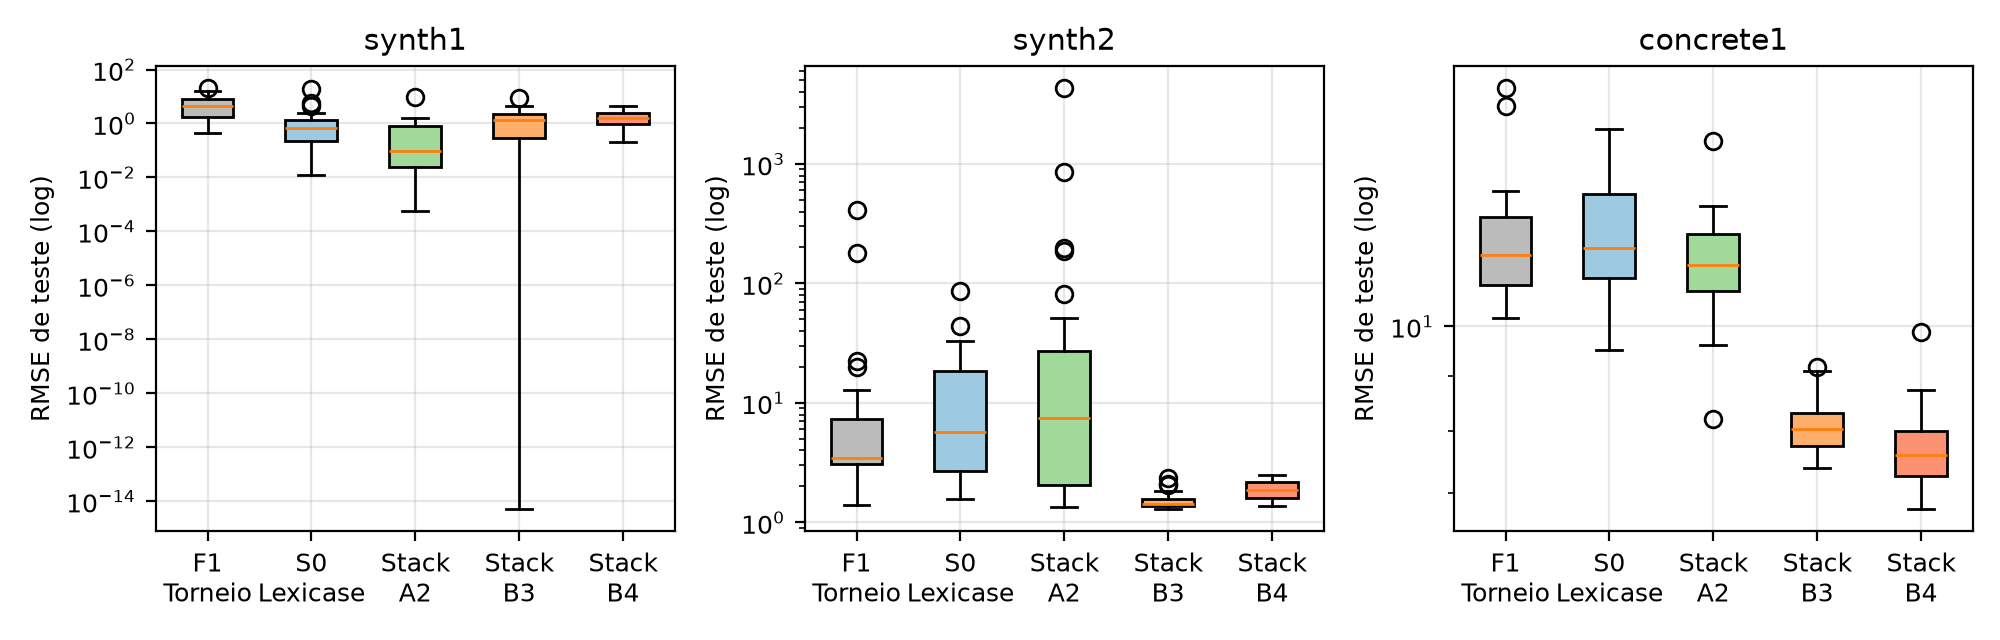
\includegraphics[width=0.92\linewidth]{f2_boxplot_bases.png}
  \caption{Distribuição do RMSE de teste (escala logarítmica) nas três bases,
           comparando o Baseline da Fase~1, o Estado Atual \cfg{S0} e as principais
           etapas de empilhamento da Fase~2.}
  \label{fig:f2_boxplot_bases}
\end{figure}

\paragraph{Por que os Especialistas Locais Falham Fora de Seus Nichos?}
A análise comparativa entre as 15 configurações elucida as razões pelas quais os
campeões especializados locais não conseguem manter a liderança global:
\begin{enumerate}
  \item \textbf{Inadequação do \cfg{Stack~A2} fora de polinômios puros:}
        O \cfg{Stack~A2} foi lapidado para a paisagem sem ruído do \code{synth1},
        operando sem \emph{Analytic Quotient} (AQ) e sem \emph{Linear Scaling}.
        Ao ser transferido para o \code{synth2}, a divisão protegida de Koza inevitavelmente
        cria polos assintóticos fora da amostra de treino, gerando um erro médio catastrófico
        de $198.35 \pm 1076.6$ (uma razão de teste $15.08\times$ pior que o \cfg{S0}).
        No \code{concrete1}, a ausência de OLS impede que os indivíduos alcancem a
        magnitude média amostral $\bar{y} \approx 35.8$ dispondo apenas de constantes
        efêmeras em $[-1, 1]$. Em decorrência disso, o \cfg{Stack~A2} cai para a
        $8^{\text{a}}$ posição em posto médio ($8.00$) e exibe uma razão geométrica de
        erro desfavorável de $1.817$.
  \item \textbf{Sobreajuste do \cfg{Stack~B4} em bases sem curvaturas não-lineares:}
        O \cfg{Stack~B4} adiciona primitivas transcendentais ($\log, \sqrt{\cdot}, \exp$).
        Embora decisivos para o \code{concrete1}, esses operadores inserem graus de
        liberdade excessivos em problemas polinomiais (\code{synth1}) e racionais
        (\code{synth2}): no \code{synth1}, essa flexibilidade espúria quadruplica a
        mediana do erro de teste de $0.093$ para $2.24$ ($p = 7.7 \times 10^{-5}$); no
        \code{synth2}, a mediana sobe de $1.43$ para $1.87$ ($p = 3.8 \times 10^{-6}$).
        Assim, seu posto médio fixa-se em $5.67$, empatado com \cfg{Stack~B1} e \cfg{Stack~B2}.
\end{enumerate}

\paragraph{A Supremacia Global do \cfg{Stack~B3}.}
Dentre todas as 15 configurações avaliadas na Fase~2 e Fase~1, o \textbf{\cfg{Stack~B3}}
emerge categoricamente como o \textbf{Melhor Modelo Global}:
\begin{enumerate}
  \item \textbf{Liderança em Posto Médio e Redução Geométrica de Erro:}
        O \cfg{Stack~B3} conquista o \textbf{menor Posto Médio global} ($\mathbf{3.67}$ nas
        médias), superando todas as outras 14 alternativas avaliadas. Sua razão
        geométrica de erro nas médias é de apenas $\mathbf{0.423}$, o que representa
        uma expressiva redução acumulada de \textbf{$57.7\%$} no erro de teste frente
        ao Estado Atual \cfg{S0}.
  \item \textbf{Desempenho Uniformemente Sólido em Todas as Paisagens:}
        \begin{itemize}
          \item No \code{synth2}, é a \textbf{configuração número 1 absoluta},
                com RMSE médio de $1.52 \pm 0.26$ e sem nenhuma divergência assintótica;
          \item No \code{concrete1}, fica a menos de $4\%$ do especialista local
                (\cfg{Stack~B4}), atingindo RMSE de $8.10 \pm 0.46$ e superando o baseline
                da Fase~1 em \textbf{30 de 30 sementes independentes} ($p_W = 1.9\times10^{-9}$);
          \item No \code{synth1}, atinge RMSE médio de $1.59 \pm 1.82$ e mediana de $1.35$,
                superando o Baseline da Fase~1 em \textbf{25 de 30 sementes} ($p_W = 7.1\times10^{-5}$).
          \item No cômputo agregado das três bases, o \cfg{Stack~B3} supera o baseline da
                Fase~1 em \textbf{85 de 90 execuções} ($94.4\%$).
        \end{itemize}
  \item \textbf{Equilíbrio Ótimo de Regularização Indutiva:}
        O \cfg{Stack~B3} é a configuração mais robusta porque combina todos os
        estabilizadores essenciais (AQ para eliminar polos; Linear Scaling para absorver
        escalas analiticamente; desduplicação para manter diversidade; parcimônia
        lexicográfica para suprimir introns; e mutação mista com perturbação gaussiana
        para ajuste contínuo de constantes), enquanto conscientemente omite operadores
        transcendetais que induzem sobreajuste em problemas polinomiais.
\end{enumerate}

Em conclusão: quando há conhecimento prévio inequívoco de uma estrutura estritamente
polinomial sem ruído, o \cfg{Stack~A2} é o especialista recomendado; para dados
multivariados complexos com curvaturas não-lineares e saturações amortecidas, o
\cfg{Stack~B4} atinge o menor erro residual; contudo, como \textbf{algoritmo de propósito
geral para regressão simbólica arbitrária sob ausência de conhecimento prévio da paisagem},
o \textbf{\cfg{Stack~B3}} constitui a recomendação ótima e definitiva deste estudo.
